\chapter{De lo clásico a lo cuántico}\label{ch:de-lo-clásico-a-lo-cuántico}


\section{La onda}\label{sec:la-onda}

Para la física, una onda consiste en la propagación de una perturbación de energía sin transporte de materia.
La magnitud física cuya perturbación se propaga se expresa como una función tanto de la posición como del tiempo
$\psi(\vec{r},t)$.

Matemáticamente se dice que una función es una onda si verifica la ecuación de ondas:
\begin{equation}
    \label{eq:ecuacion-onda}
    \nabla^2\psi(\vec {r},t)=\frac {1}{v^2}\frac{\partial^2\psi}{\partial t^2}(\vec {r},t)
\end{equation}
donde $v$ es la velocidad de propagación de la perturbación.

\subsection{elementos de una onda}\label{subsec:elementos-de-una-onda}

\begin{description}
    \item[Cresta.] El punto de máxima separación con respecto de su posición de reposo.
    \item[Valle.] El punto de máxima elongación de la onda, en sentido opuesto a la cresta.
    \item[Amplitud ($\amplitud$).] La distancia vertical desde una cresta hasta el punto de equilibrio.
    \item[Longitud de onda ($\longonda$).] La distancia entre dos crestas consecutivas.
    \item[Número de onda angular ($\longondaangular$).] La inversa de la longitud de onda en radianes.
    \item[Periodo ($\periodo$).] El tiempo empleado en completar una longitud de onda.
    \item[Frecuencia ($\frecuencia$).] El número de periodos por unidad de tiempo.
    \item[Frecuencia angular ($\frecuenciaangular$).] La frecuencia en radianes por segundo.
    \item[Fase ($\fase$).] El mínimo valor que hace cíclica la posición.
    \item[Velocidad de fase ($v_f$).] La velocidad a la que se propaga el movimiento ondulatorio.
    \item[Velocidad de grupo ($v_g$).] La velocidad a la que se propaga las variaciones de la amplitud.
\end{description}
Podemos ver algunos de estos conceptos en la figura~\eqref{fig:elementos-onda}.
Aplicando las definiciones anteriores, tenemos
\begin{align*}
    \longondaangular &= \frac{2\pi}{\longonda} & \frecuencia &=\frac{1}{\periodo} \\
    v_f &= \frac{\longonda}{\periodo}=\frac{\frecuencia}{\longondaangular} & \frecuenciaangular &= 2\pi\frecuencia
\end{align*}

\begin{figure}[htbp]
    \centering
    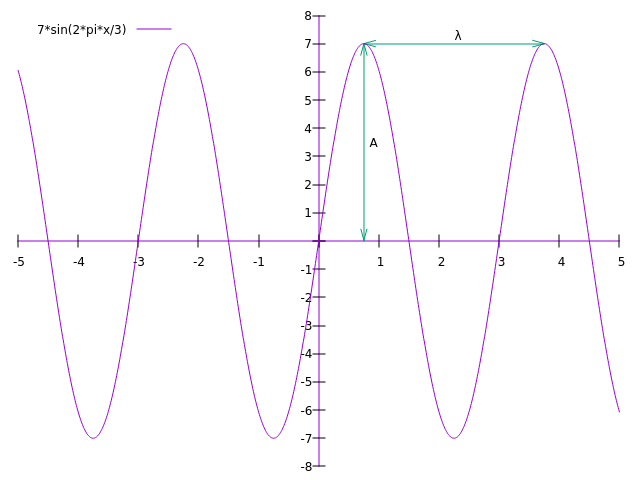
\includegraphics[width=0.6\textwidth]{sin}
    \caption{elementos de una onda}
    \label{fig:elementos-onda}
\end{figure}

\subsection{Soluciones a la ecuación de onda}\label{subsec:soluciones-a-la-ecuación-de-onda}
La solución más sencilla a la ecuación de ondas es considerar una onda plana que se desplaza longitudinalmente en la dirección de la onda, donde si situamos el sistema de referencia en un punto de equilibrio tenemos la solución:
\begin{equation}
    \label{eq:solucion-ecuacion-ondas-simple}
    \psi(x,t)=\amplitud\sin(\longondaangular x - \frecuenciaangular t)
\end{equation}

Pero la luz en una onda electro-magnética y como ya apreció Maxwell, el campo magnético aporta una componente a las ecuaciones en forma de onda compleja, y en este caso, la solución más sencilla de onda electro-magnética plana que se desplaza longitudinalmente en la dirección de la onda es:
\begin{equation}
    \label{eq:solucion-ecuacion-ondas-complejas-simple}
    \psi(x,t)=\amplitud e^{i(\longondaangular x - \frecuenciaangular t)}
\end{equation}


\section{Dualidad onda-partícula de De Broglie}\label{sec:dualidad-onda-partícula-de-de-broglie}

Si los fotones son partículas y ondas a la vez, podemos usar el postulado de la mecánica relativista de Einstein para partículas, y a la vez, el postulado de Planck para ondas.

\begin{postulate}[Valor de la energía de las ecuaciones de Einstein]
    \begin{equation}
        \label{eq:energia-einstein}
        \energia=m{\speedoflightsymbol}^2=p\speedoflightsymbol
    \end{equation}
\end{postulate}

\begin{postulate}[Valor de la energía de las ecuaciones de Planck]
    \begin{equation}
        \label{eq:energia-planck}
        \energia=\plancksymbol\frecuencia=\frac{\plancksymbol\speedoflightsymbol}{\longonda}
    \end{equation}
\end{postulate}

Así pues igualando ambas energías obtenemos la relación para cada partícula entre su momento y su longitud de onda:
\begin{postulate}[Relación entre longitud de onda y momento de De Broglie]
    \begin{equation}
        \label{eq:dualidad-de-broglie}
        \longonda=\frac{\plancksymbol}{p}
    \end{equation}
\end{postulate}

\begin{example}
    Calcular la longitud de onda de una persona de masa $\mass{8}$ cuando anda a una velocidad de $\velocity{45}$.

    La persona tiene un momento de $\momento{8*45*1000/3600=1000}$.
    Así que la longitud de onda asociada es de $\longonda=\frac{6,6256*\tento{-34}}{1000}=\espacio{6,6256*\tento{-37}}$.
\end{example}

\begin{note}
    La longitud de onda más pequeña que actualmente podemos observar es del orden de $\espacio{\tento{-20}}$ con el \textbf{Cherenkov telescope array}.
\end{note}

\subsection{Conclusiones}\label{subsec:conclusiones}
Usando la nueva relación entre longitud de onda y momento, podemos obtener las siguientes igualdades:
\begin{align}
    \label{eq:k-debroglie}
    \longondaangular &= \frac{2\pi}{\longonda}\by{\ref{eq:dualidad-de-broglie}}\frac{2\pi p}{\plancksymbol}=\frac{p}{\planckbarsymbol}\\
    \label{eq:omega-planck}
    \frecuenciaangular &= 2\pi\frecuencia\by{\ref{eq:energia-planck}}2\pi\frac{\energia}{\plancksymbol}=\frac{\energia}{\planckbarsymbol} \\
    \label{eq:omega_debroglie}
    \frecuenciaangular &\by{\ref{eq:omega-planck}}\frac{\energia}{\planckbarsymbol}=\frac{p^2}{2m\planckbarsymbol}\by{\ref{eq:dualidad-de-broglie}}\frac{\plancksymbol^2}{\longonda^2 2m\planckbarsymbol}=\frac{2\pi h}{\lambda^2 2m}=\frac{\planckbarsymbol \longondaangular^2}{2m}\\
    \label{eq:frecuencia_debroglie}
    \nu &\by{\ref{eq:energia-planck}}\frac{\energia}{\plancksymbol}=\frac{p^2}{2m\plancksymbol}\by{\ref{eq:dualidad-de-broglie}}\frac{\plancksymbol^2}{2m\plancksymbol\longonda^2}=\frac{\plancksymbol}{2m\longonda^{2}}
\end{align}

\subsection{Solución de onda momento-energía}\label{subsec:solucion-de-onda-momento-energia}
Una consecuencia interesante de la dualidad onda-partícula de De Blogie, es poder expresar la solución de onda electro-magnética en función de su energía y su momento.

\begin{equation}
    \label{eq:ecuacion_onda_momento_energia}
    \psi(x,t)=\amplitud e^{i(\longondaangular x - \frecuenciaangular t)}\by{\ref{eq:omega-planck} y~\ref{eq:k-debroglie}}\amplitud e^{i(\frac{p}{\planckbarsymbol}x - \frac{\energia}{\planckbarsymbol} t)}=\amplitud e^{i(\planckbarsymbol^{-1}(p x - \energia t))}
\end{equation}

\subsection{Desarrollo de la ecuación de Schröndiger}\label{subsec:desarrollo-de-la-ecuación-de-schrondiger}

Partimos de la solución de onda momento-energía~\eqref{eq:ecuacion_onda_momento_energia}, calculamos la derivada parcial respecto del tiempo y la segunda derivada parcial respecto del espacio dos veces y recordamos que la energia es la suma de la energía cinética y energía potencial.
\begin{equation}
    \label{eq:pre-schrondiger}
    \frac{\partial\psi}{\partial x}=\frac{ip}{\planckbarsymbol}\psi\so\frac{\partial^2\psi}{\partial x^2}=\frac{-p^2}{\planckbarsymbol^2}\psi
\end{equation}

\begin{equation}
    \label{eq:desarrollo-ecuacion-schrodinger}
    \frac{\partial\psi}{\partial t}=\frac{i\energia}{\planckbarsymbol}\psi=\frac{ip^2}{2m\planckbarsymbol}\psi+\frac{iV}{\planckbarsymbol}\psi=\frac{i\planckbarsymbol}{2m}\frac{p^2}{\planckbarsymbol^2}\psi+\frac{iV}{\planckbarsymbol}\psi\by{\ref{eq:pre-schrondiger}}\frac{-i\planckbarsymbol}{2m}\frac{\partial^2\psi}{\partial x^2}+\frac{iV}{\planckbarsymbol}\psi
\end{equation}
